\section{Experimentation}
\label{sec:experimentation}

\noindent In order to assess the feasibility of our proposal we build a prototype called \emph{Topicalizer}, which implements the mechanisms described throughout this report, for the particular case of SOAP services. 

The implemented system receives as input a list of URIs from real WSDL interfaces available online. The system retrieves each WSDL and processes it by following the techniques outlined in sections \ref{subsub:soap} and \ref{subsub:Service-documentation-cleaning} and stores its relevant information into a service registry. In doing this processing a stream of documents is generated, each one of them containing information related to a specific SOAP service operation. Then the stream of documents is categorized based on the document's content by applying the \emph{online LDA} algorithm as described in sections \ref{subsub:The-Latent-Dirichlet} and \ref{subsub:Application-of-LDA}. Such categorization arranges semantically-related documents into clusters which are defined by a weighted set of terms, that in turn become annotations on the operations that each document represents. The information gathered from the categorization process is specified in RDFS---conforming to the data model defined in section \ref{subsub:RDF-spec-of-KNOWEB}---and stored into an RDF triplestore.

The system architecture is depicted in Figure \ref{prototype-architecture}:

\begin{figure}
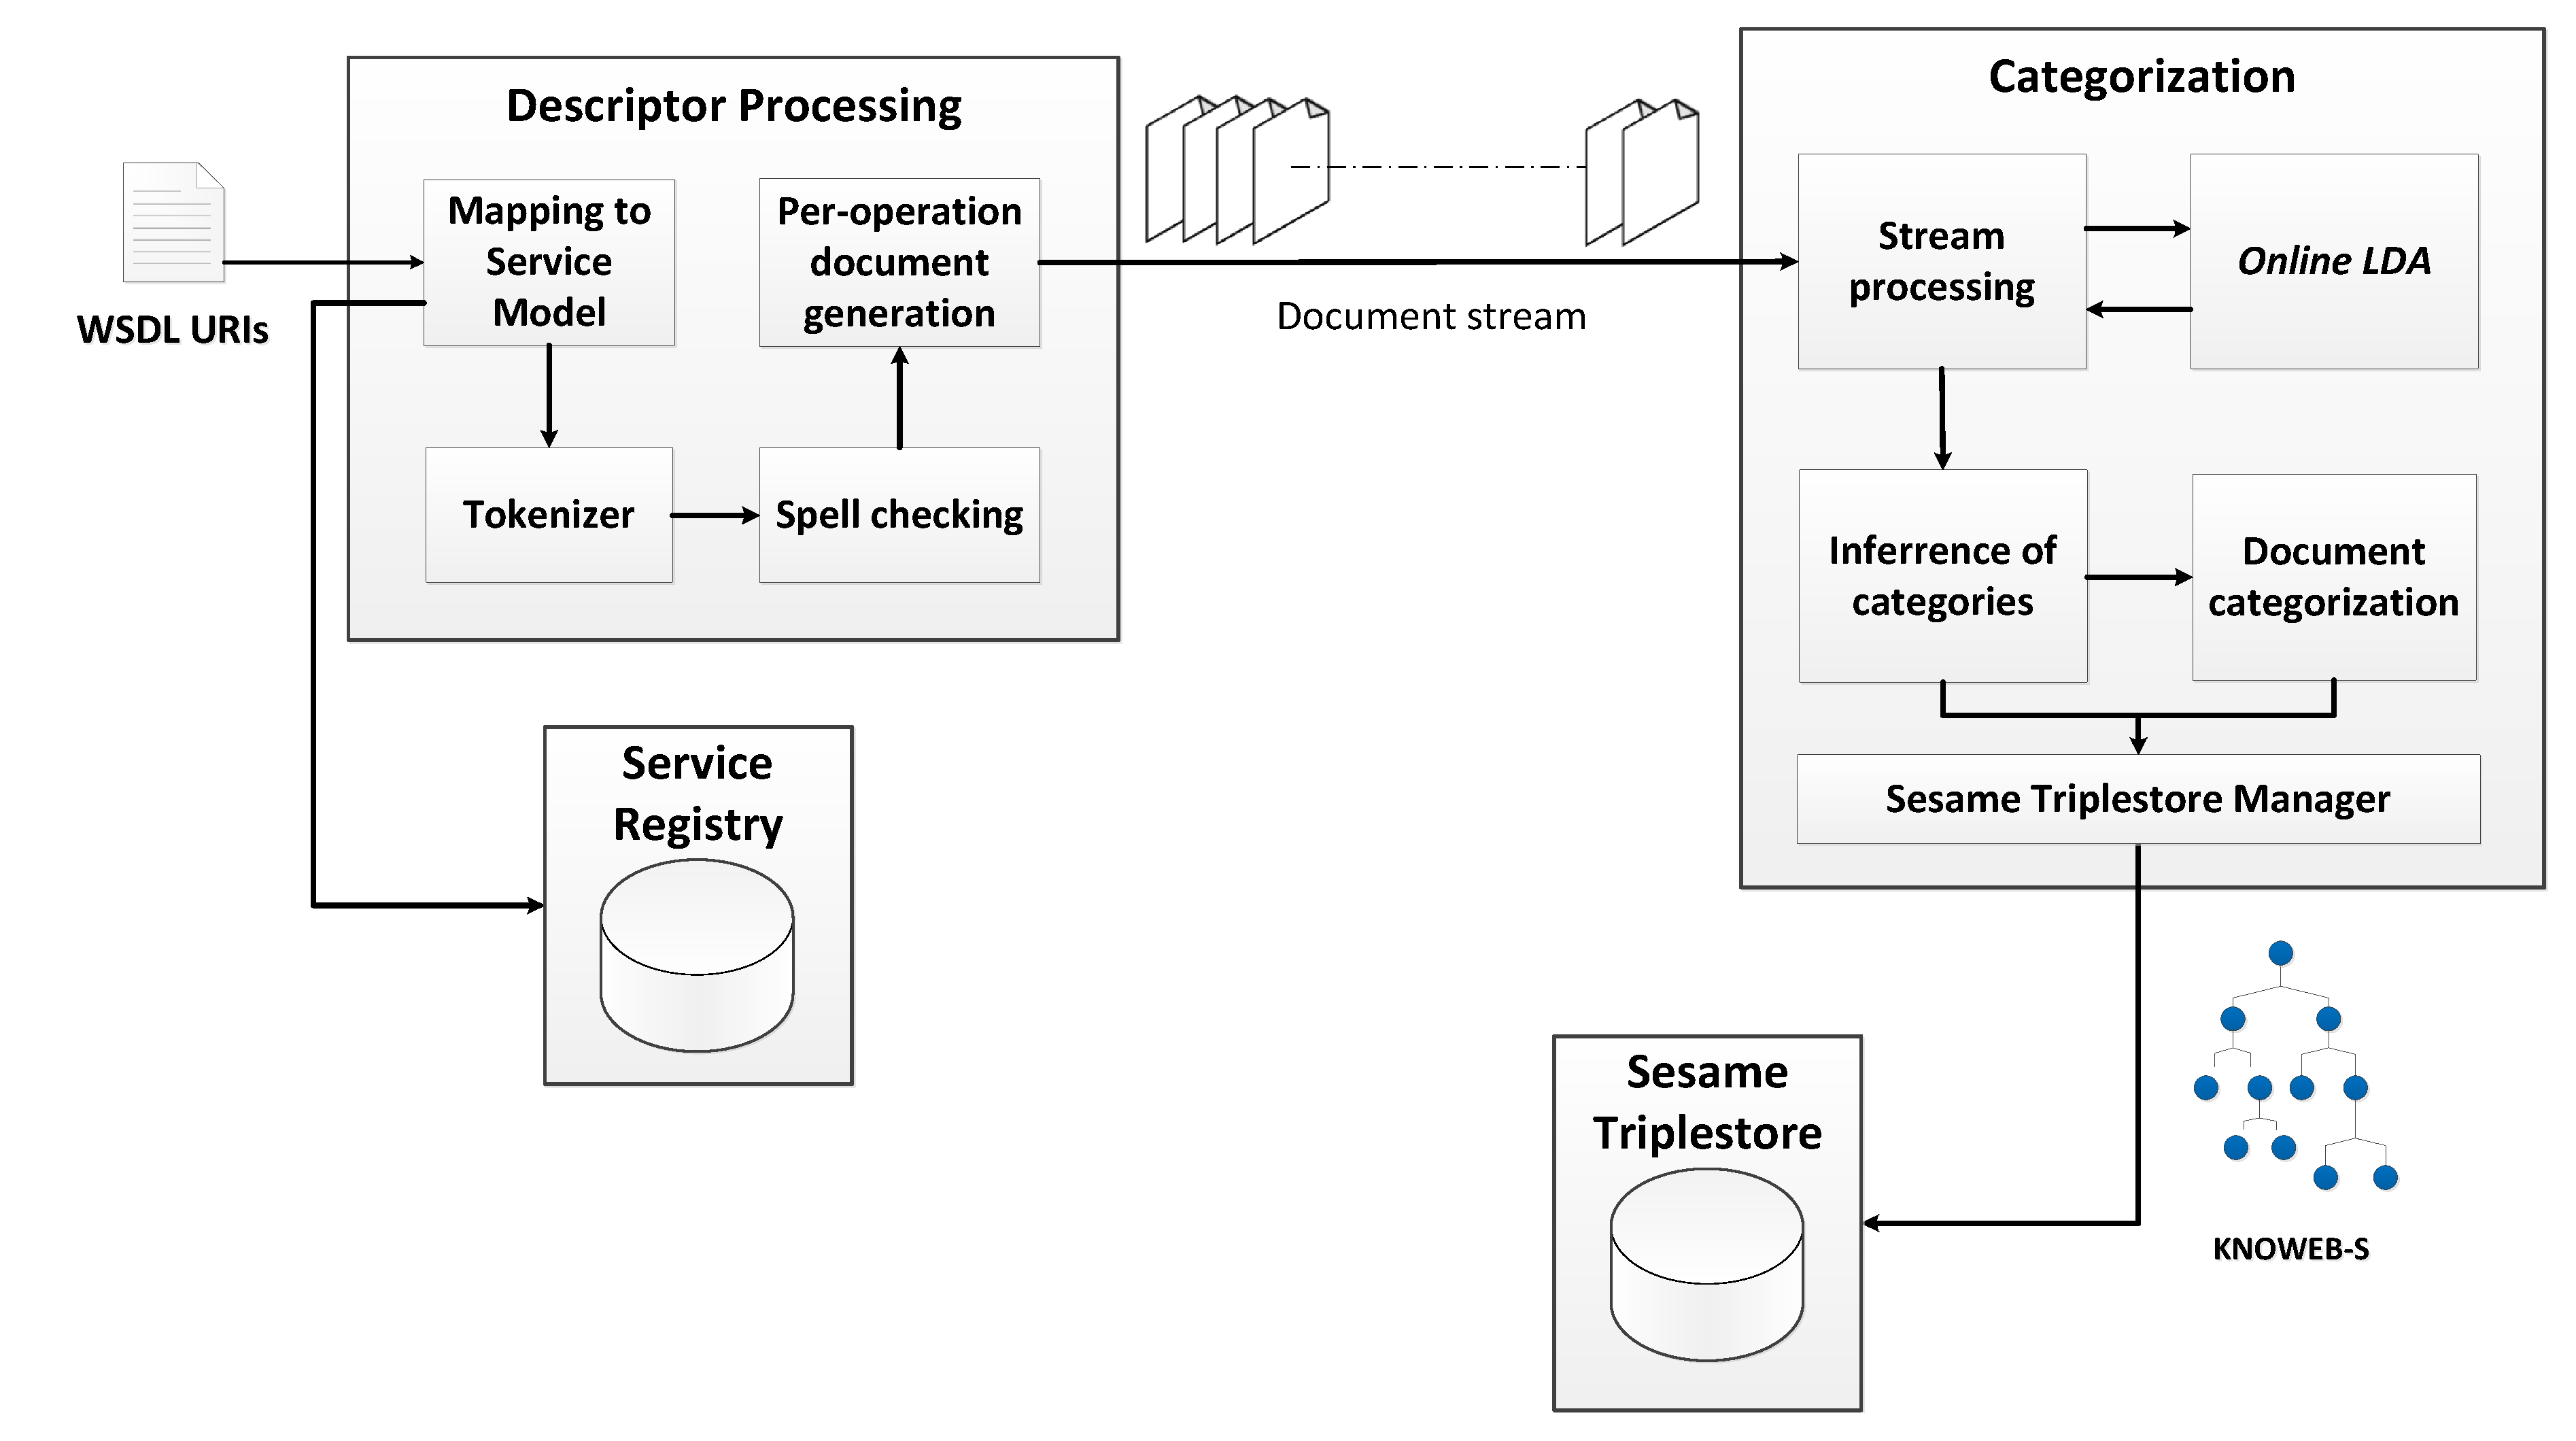
\includegraphics[scale=0.20]{images/prototype-architecture}

\caption{Architecture of Topicalizer.}
\label{prototype-architecture}

\end{figure}


Each one of the components comprising the architecture of Topicalizer are described below:
\begin{itemize}

\item \emph{Descriptor processing}: this module of the architecture is in charge of reading the list of WSDL URIs, accessing each descriptor via HTTP request, loading it into memory, mapping it into the SOAP service model defined in section \ref{subsub:soap} (see Figure \ref{wsdl-Simplified}) and storing the mapped information into a service registry. Once these initial procedures have been performed, this module applies tokenization and spell checking techniques---described in section \ref{subsub:Service-documentation-cleaning}---on the content of each descriptor and finally, for every operation of the processed descriptor it generates a document in plain text containing: (\emph{i}) the operation name, (\emph{ii}) its description in natural language, (\emph{iii}) the name of the service it belongs to, and (\emph{iv}) its input/output parameters. This module was implemented in Java, using its persistence API (JPA) and the \emph{EasyWSDL} library for WSDL manipulation \footnote{Available at: \href{http://easywsdl.ow2.org/}{http://easywsdl.ow2.org/}}.

\item \emph{Service registry}: consists of a relational database, implemented in MySQL. The entity-relationship model of this database matches the service model described in section \ref{subsub:soap}. 

\item \emph{Categorization}: this component receives the stream of documents generated by the descriptor processing module, then splits it in small-sized batches and delivers them to the implementation of online LDA, which is based on an adaptation of an existing application developed by Matthew D. Hoffman, one of the authors of the mentioned algorithm \cite{Hoffman:2010}. Once the processing of the stream of documents is completed, the derived results are interpreted for establishing the set of terms that compose each category---task performed by the \emph{inference of categories }sub-module---as well as the group of documents included in each one of them---which is defined by the \emph{document categorization} sub-module. The derived arrangement of categories, documents and terms, is mapped into the KNOWEB-S data model and stored into a RDF triplestore provided by the \emph{Sesame} openRDF framework \footnote{Available at: \href{http://www.openrdf.org/index.jsp}{http://www.openrdf.org/index.jsp}}. This component of the architecture was developed in Python, using the \emph{numpy}, \emph{urllib2} and \emph{httplib2} libraries.

\item \emph{Sesame Triplestore}: It is an HTTP repository for RDF triples, hosted in an Apache Tomcat web server. This repository stores the KNOWEB-S taxonomy generated by the previous Categorization component. Sesame allows the retrieval and manipulation of the information encoded in KNOWEB-S by using SPARQL queries.
\end{itemize}

The whole prototype is executed by using a bash script, which receives as input the path of a text file containing the list of WSDL URIs. The prototype also generates two documents in \emph{csv} format for specifying: (1) the terms that define each of the identified categories along with their associated relevance value, and (2) the per-document category proportions for each of the processed documents (i.e. SOAP service operations).  
A description of the source code structure of the prototype is available at \href{https://github.com/LeandroOrdonez/Topicalizer}{https://github.com/LeandroOrdonez/Topicalizer}.